\section{Methodology}
\label{sec-methodology}


%Describe your approach and design
%Instead of simply explaining what you ended up doing, show why you made such
%design decisions / how what the trade-offs are.

Describe the general computer architecture design that we are considering for
memory encryption. Generally use AES-CTR mode encryption

\subsection{Model}

\begin{figure}
  \centering
  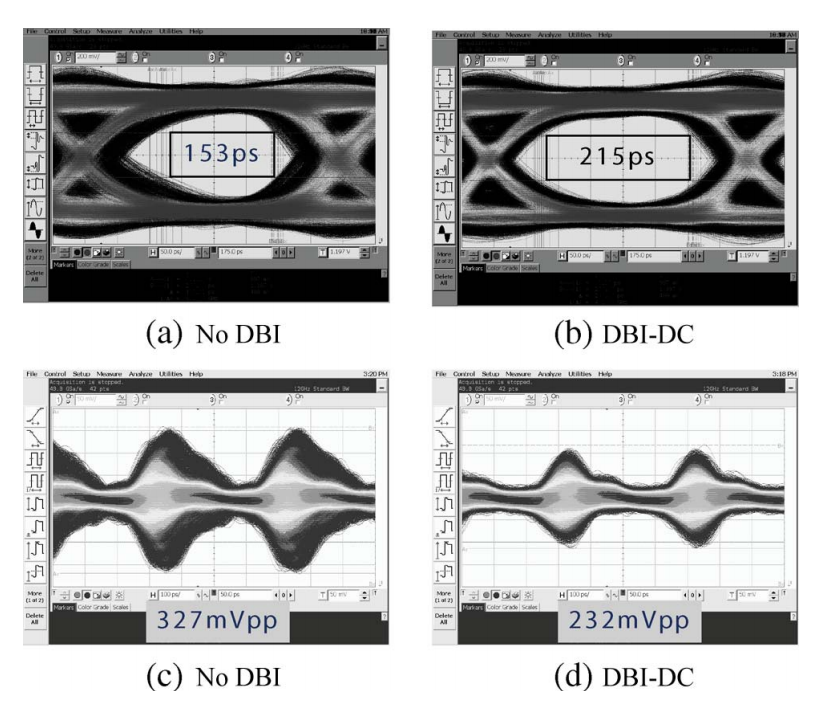
\includegraphics[width=0.3\textwidth]{figs/dbi-dc}
  \caption{DBI DC Impact \cite{hollis}}
  \label{fig:dbi-dc}
\end{figure}

\begin{enumerate}
  \item Introduce equation
    $$ P_t = A \times P_{dc} + B \times P_{ac}$$
  \item Talk about encrypted data : A = 0.5, B = 0.5 : Assumption that Data is
    Completely random once encrypted
  \item Say that DBI aims to reduce A, B by using program structure
\end{enumerate}

\subsection{Experimental Setup}
\begin{enumerate}
  \item PIN - dynamic binary instrumentaiton tool : describe cache settings
  \item Computer architecture analysis tool
  \item MiBench - Justify why MiBench (mobile) ---- SPEC is not as good
  \item DRAMSim - Did not work for us.
  \item Python Script to analyze the loads and stores from the trace outptted
    from PIN
\end{enumerate}
